\label{sec:introducao}

A superlotação dos serviços de urgência e emergência é um problema persistente dos sistemas públicos de saúde, com efeitos documentados sobre a segurança do paciente, a qualidade assistencial, o tempo de espera e o custo operacional \cite{savioli2022, pearce2023}. No Brasil, a superlotação das unidades de emergência é descrita como uma realidade com tendência de piora, que compromete a segurança dos pacientes e as condições de trabalho das equipes \cite{freitas2024}. Unidades de Pronto Atendimento (UPA) e Unidades Básicas de Saúde (UBS) absorvem demandas de diferentes níveis de complexidade, inclusive queixas que poderiam ser resolvidas por outros canais da rede.

Entre os fatores de entrada desse cenário está a presença de pacientes de baixo risco clínico. No Protocolo de Manchester, os pacientes classificados como verde e azul não demandam atendimento imediato e têm tempos máximos de espera de 120 e 240 minutos a partir da classificação \cite{stormversloot2014}. Em um departamento de emergência pediátrica de Viena, que atingiu cerca de 25 mil atendimentos anuais, 95\% dos pacientes procuravam o serviço por conta própria e 75\% eram classificados nos níveis verde e azul \cite{sorznechay2025}. A busca por esses serviços está associada à conveniência, à ansiedade em relação à própria saúde e à dificuldade de acesso oportuno a outros pontos da rede \cite{schmiedhofer2016}.

Depois da expansão da saúde digital durante a pandemia de COVID-19 \cite{donida2021, ndayishimiye2023}, a telessaúde ganhou marco legal permanente pela Lei n.º 14.510/2022, que assegura ao paciente o direito de recusar o atendimento a distância e de ser atendido presencialmente sempre que solicitar \cite{lei14510}. A Resolução CFM n.º 2.314/2022 regulamentou a telemedicina, exigiu consentimento explícito do paciente e manteve com o médico a prerrogativa de indicar o atendimento presencial \cite{cfm2314}. No mesmo período, quiosques de autoatendimento passaram a ser usados em serviços de emergência, com ganhos concentrados em etapas como o registro e a pré-triagem \cite{joseph2023}.

O uso isolado dessas tecnologias, porém, não resolve o problema. A autotriagem eletrônica apresentou baixa concordância com a triagem feita por enfermeiros em dois serviços de emergência do Reino Unido \cite{dickson2022}, o que desaconselha transferir a classificação de risco para o próprio dispositivo. Além disso, qualquer solução que pretenda se integrar ao Sistema Único de Saúde (SUS) precisa observar os padrões nacionais de interoperabilidade, publicados para a Rede Nacional de Dados em Saúde (RNDS), e as regras de proteção de dados pessoais sensíveis da Lei Geral de Proteção de Dados Pessoais (LGPD) \cite{portaria1434, lgpd2018, leme2020}.

Do lado da engenharia de software, uma revisão sistemática sobre arquiteturas de telemedicina identificou a recorrência de segurança, interoperabilidade e escalabilidade como preocupações centrais, mas com tratamento superficial dos requisitos regulatórios \cite{jat2024}. A arquitetura modular baseada em HL7 FHIR proposta por Gøeg et al. mostrou que um núcleo de baixo acoplamento é viável, mas sua avaliação clínica ficou como trabalho futuro e o contexto era o da Dinamarca \cite{goeg2018}. Faltam propostas que articulem, em uma mesma arquitetura, a classificação de risco presencial, o atendimento remoto no próprio ambiente da unidade e a integração com os perfis e terminologias da rede nacional brasileira.

A proposta deste trabalho parte desse ponto. O paciente classificado como de baixo risco na triagem presencial pode ser atendido por um médico remoto, por vídeo, em um totem instalado na própria unidade, sem sair do alcance da equipe de enfermagem e sem perder a possibilidade de voltar ao atendimento presencial. A Figura~\ref{fig:fluxo} resume esse fluxo na visão de quem participa dele.

\begin{figure}[H]
\centering
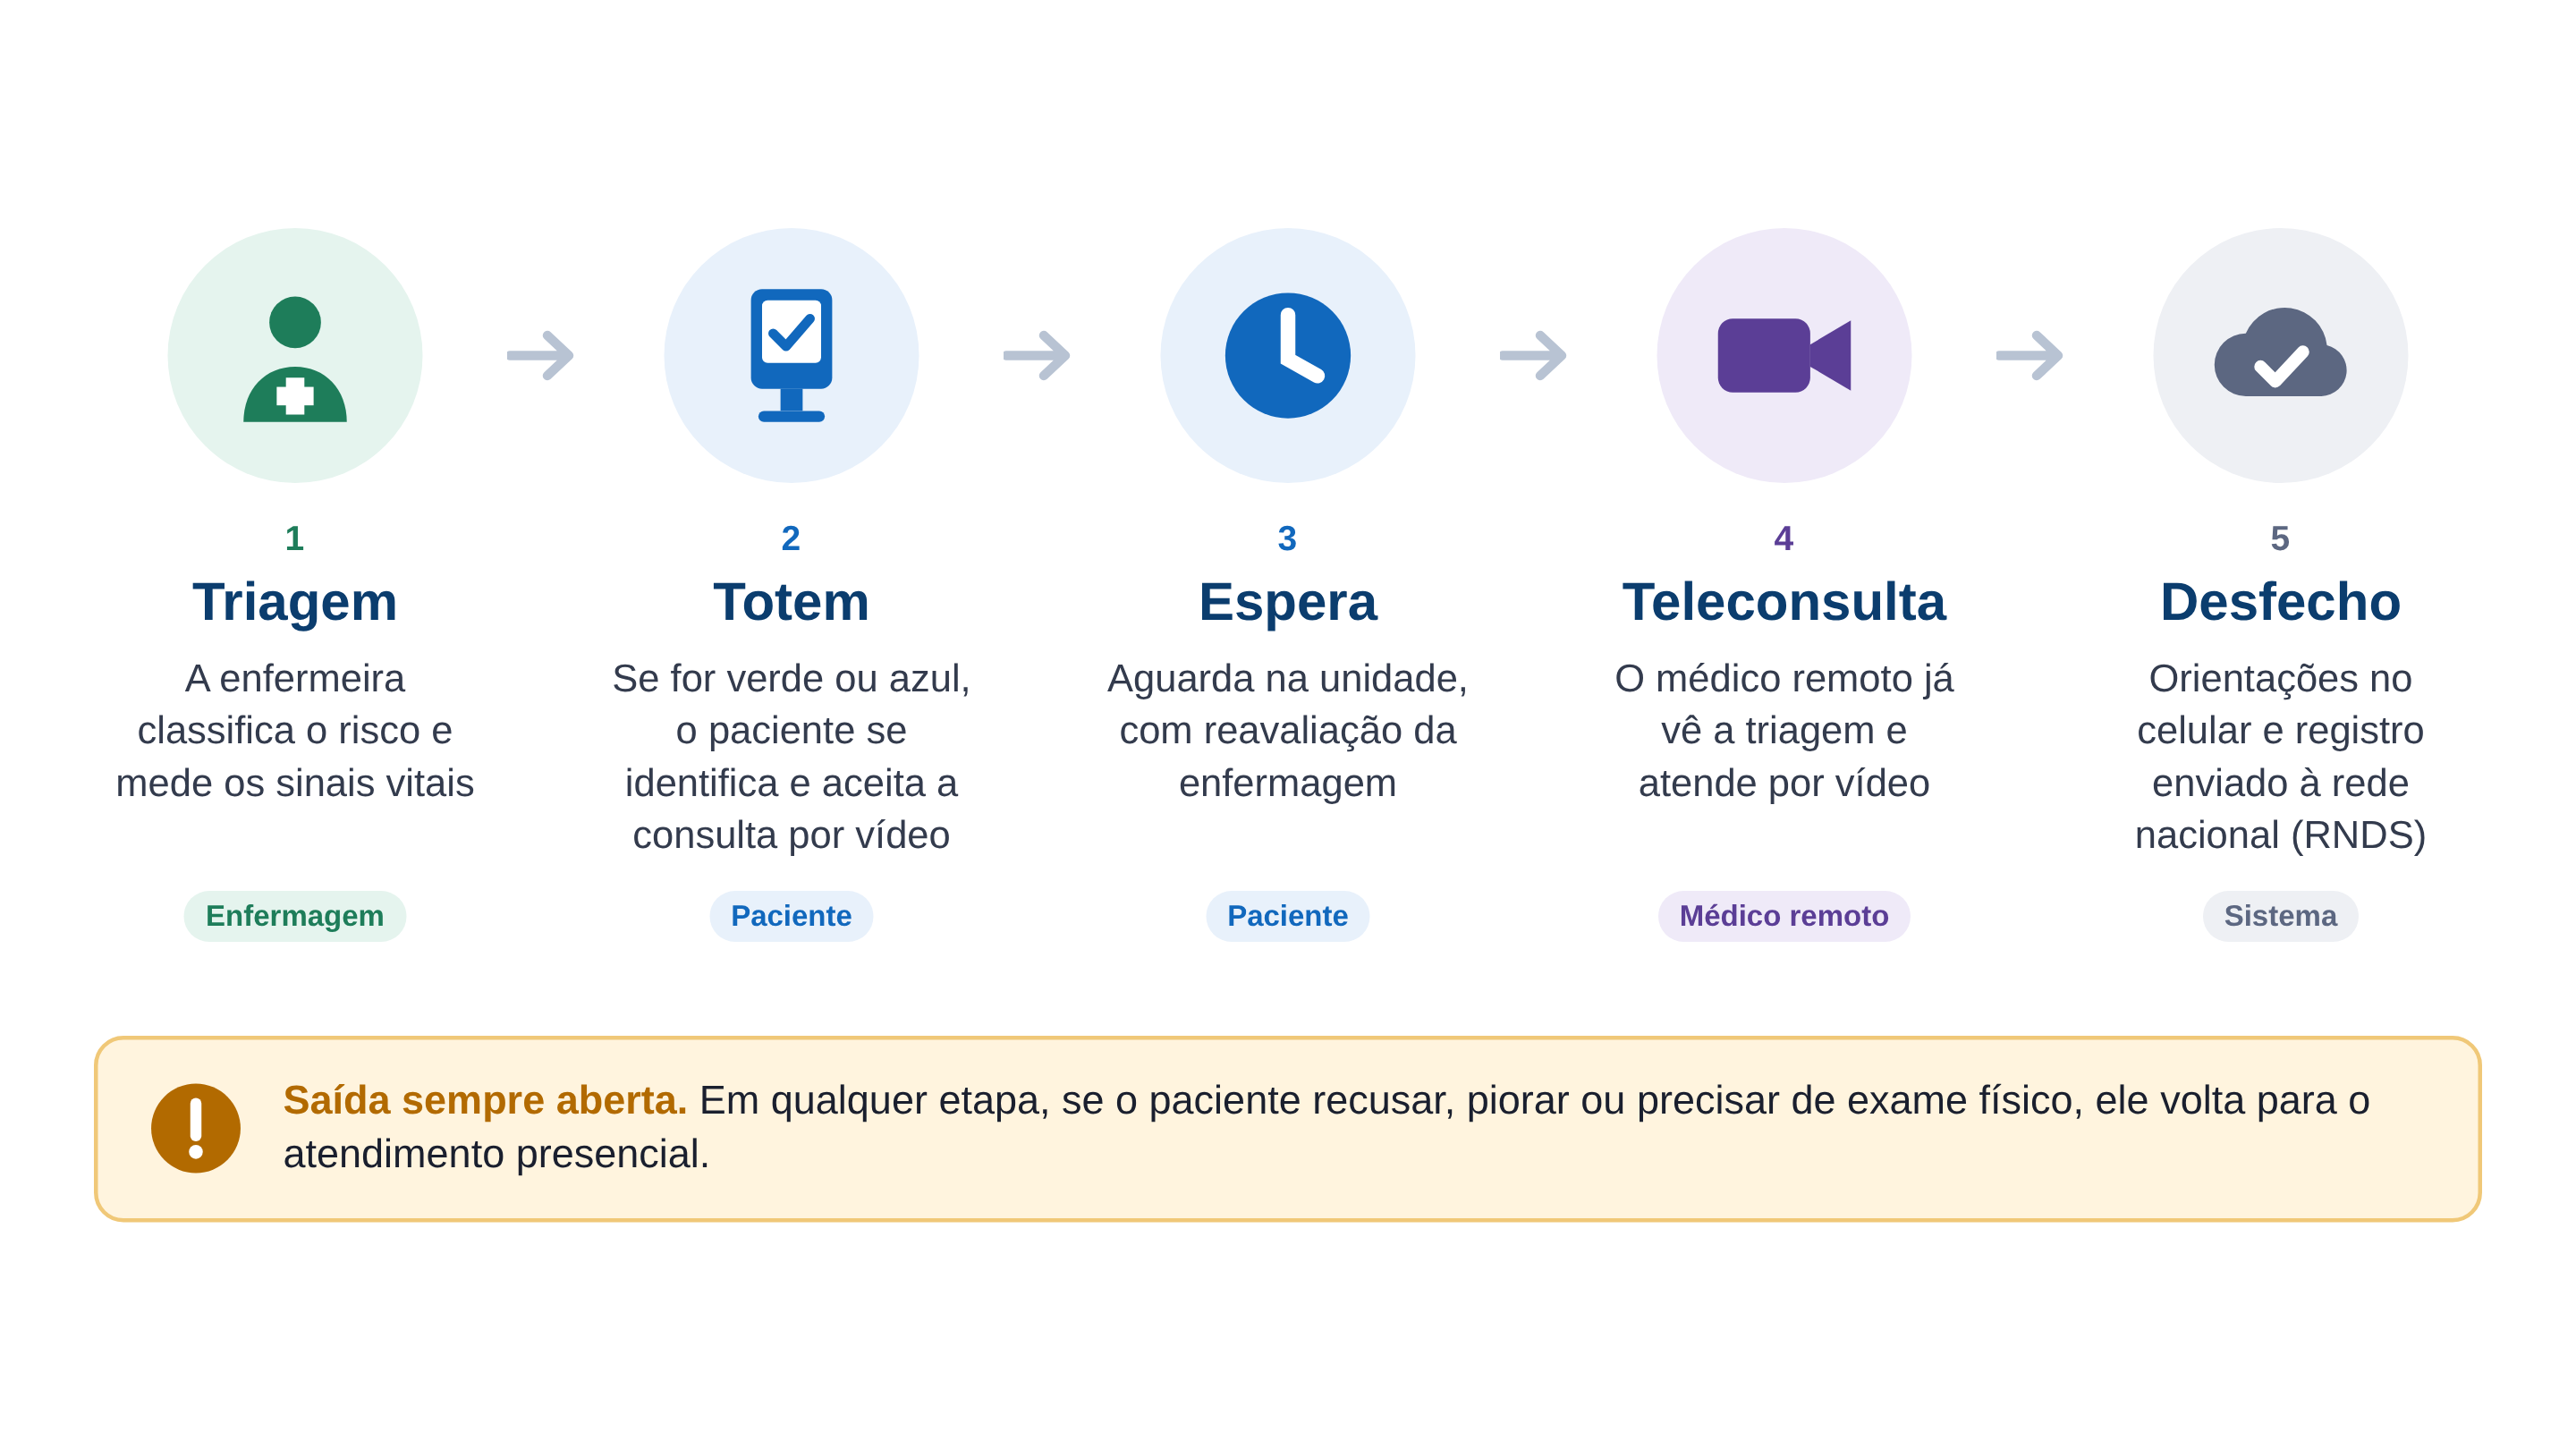
\includegraphics[width=\textwidth]{figuras/fluxo-atendimento.png}
\caption{Visão geral do atendimento por teleconsulta no totem}
\label{fig:fluxo}
\fonte{Elaboração própria.}
\end{figure}

\subsecao{Problema e questão de pesquisa}

O problema tratado neste trabalho é a ausência de uma arquitetura de software, documentada de forma rastreável, que permita oferecer teleconsulta em totem a pacientes já classificados como de baixo risco, sem transferir ao dispositivo a responsabilidade pela classificação, com critérios clínicos explícitos de elegibilidade e retorno ao atendimento presencial, e com aderência demonstrável aos padrões nacionais de interoperabilidade e à legislação de proteção de dados.

A questão que orienta o trabalho é: \textit{como estruturar uma arquitetura de software que viabilize a teleconsulta em totem para pacientes já triados como de baixo risco, de forma rastreável às evidências, segura do ponto de vista assistencial e aderente aos padrões nacionais de interoperabilidade e à proteção de dados?}

\subsecao{Justificativa}

A relevância do trabalho tem três dimensões. A primeira é assistencial: um canal remoto dentro da própria unidade mantém o paciente próximo da equipe de enfermagem, o que permite reavaliação e retorno imediato ao atendimento presencial em caso de piora, diferentemente da teleconsulta domiciliar. A segunda é regulatória: a Portaria GM/MS n.º 3.691/2024, que instituiu a Ação Estratégica SUS Digital - Telessaúde, exige que as plataformas de telessaúde sejam interoperáveis com a RNDS e com os prontuários eletrônicos \cite{portaria3691}, e a LGPD trata dados de saúde como dados pessoais sensíveis \cite{lgpd2018}. A terceira é técnica: a literatura de arquitetura de software para telemedicina tende a declarar a adoção do FHIR sem especificar perfis, terminologias, autenticação e tratamento de erros, que são justamente os pontos que decidem se um sistema consegue ou não trocar dados com a rede nacional \cite{jat2024}.

O trabalho também responde a uma lacuna de método. A versão preliminar desta proposta, apresentada como artigo no XXI Congresso Brasileiro de Informática em Saúde (CBIS 2026), foi revisada a partir de pareceres que pediram rastreabilidade entre fontes e requisitos, critérios clínicos além da cor do Protocolo de Manchester, especificação precisa da integração com a RNDS, distinção entre base legal e consentimento e descrição de como a proposta conceitual foi avaliada. Esta monografia incorpora essas revisões e amplia a fundamentação, a especificação e a avaliação analítica.

\subsecao{Objetivos}

\subsubsecao{Objetivo geral}

Propor e avaliar analiticamente uma arquitetura de software para telemedicina embarcada em totens de autoatendimento, voltada ao atendimento pós-triagem de pacientes de baixo risco em unidades públicas de saúde.

\subsubsecao{Objetivos específicos}

\begin{enumerate}
    \item Levantar, por revisão narrativa protocolada, os condicionantes assistenciais, regulatórios e técnicos do atendimento remoto de pacientes de baixo risco no SUS.
    \item Derivar requisitos funcionais e não funcionais rastreáveis às fontes, aos riscos que endereçam e aos componentes que os atendem.
    \item Especificar critérios clínicos de elegibilidade, reavaliação e retorno seguro ao fluxo presencial, tratando a classificação de risco como condição necessária, mas não suficiente.
    \item Modelar a arquitetura em camadas e documentá-la com o modelo C4 e com diagrama de sequência.
    \item Especificar a integração com a RNDS em termos de modelo de informação, perfis, terminologias, autenticação, validação e tratamento de erros.
    \item Avaliar a proposta por análise de cenários de qualidade, verificação de conformidade normativa e análise de cobertura entre requisitos e componentes.
\end{enumerate}

\subsecao{Contribuições}

As contribuições do trabalho são quatro: (i) uma matriz de rastreabilidade entre fontes, requisitos, riscos e componentes; (ii) a especificação de critérios clínicos que condicionam o uso do canal remoto, incluindo reavaliação periódica e reconhecimento de deterioração; (iii) o mapeamento da integração com a RNDS a partir do modelo de informação do Registro de Atendimento Clínico (RAC) e da documentação técnica oficial; e (iv) uma avaliação analítica prévia, com lista de verificação de conformidade e cenários de qualidade, cujos limites são declarados explicitamente.

\subsecao{Delimitação}

O trabalho é uma proposição arquitetural. A solução não foi prototipada, implantada nem testada com pacientes ou profissionais. Por isso, nenhuma conclusão sobre redução da superlotação, resolutividade, tempo de espera ou segurança operacional é derivada dele. O alcance das conclusões restringe-se à consistência interna do projeto, à sua aderência documental às normas e ao seu potencial de integração futura ao ecossistema digital do SUS.

\subsecao{Estrutura do trabalho}

O Capítulo 2 apresenta o referencial teórico: superlotação, perfil dos pacientes de baixo risco, Protocolo de Manchester, telemedicina e seu marco regulatório, quiosques e autotriagem, proteção de dados, ecossistema digital do SUS, arquitetura de software para telemedicina e trabalhos correlatos. O Capítulo 3 descreve a metodologia, orientada por \textit{Design Science Research}. O Capítulo 4 apresenta e discute os resultados: requisitos e rastreabilidade, arquitetura, critérios clínicos, interoperabilidade, proteção de dados, decisões arquiteturais e avaliação analítica. O Capítulo 5 traz as conclusões e os trabalhos futuros. Os apêndices reúnem a lista de verificação de conformidade, a matriz de cobertura e exemplos ilustrativos das requisições à RNDS.
